\documentclass[11pt]{article}

\usepackage[french]{babel}
\usepackage[utf8]{inputenc}
\usepackage{tikz}
\usepackage{pgf}
\usetikzlibrary{arrows,automata}
\usepackage[left=2cm, right=2cm]{geometry}
\usepackage{amsmath,amsfonts,amssymb}
\usepackage{listings}
\usepackage{graphicx}
\usepackage{multirow}
\usepackage{hyperref} % Required for links
\usepackage{enumitem}
\date{}
\begin{document}

\def \ETScourse {ELE778-01 - Intelligence artificielle: réseaux neuroniques
et systèmes experts}
\def \ETStitle {Laboratoire 2}
\def \ETSprof  {Cynthia \textsc{Moussa}}
\def \ETSauthA {Liam \textsc{Beguin}\\\emph{BEGL02129304}}
\def \ETSauthB {Louis \textsc{Laporte}\\\emph{LAPL14128903}}
% Author : liambeguin
%
% To use this page add the following in your main page:
%
%\def \ETScourse {ELE430-01 - Conception des filtres Analogiques}
%\def \ETStitle {Laboratoire 2}
%\def \ETSprof {François \textsc{Gourlay}}
%\def \ETSauthA {Liam \textsc{Beguin}\\\emph{BEGL02129304}}
%\def \ETSauthB {Olivier \textsc{Belisle}\\\emph{BELO21098902}}
%\def \ETSauthC {bar}
%% Author : liambeguin
%
% To use this page add the following in your main page:
%
%\def \ETScourse {ELE430-01 - Conception des filtres Analogiques}
%\def \ETStitle {Laboratoire 2}
%\def \ETSprof {François \textsc{Gourlay}}
%\def \ETSauthA {Liam \textsc{Beguin}\\\emph{BEGL02129304}}
%\def \ETSauthB {Olivier \textsc{Belisle}\\\emph{BELO21098902}}
%\def \ETSauthC {bar}
%% Author : liambeguin
%
% To use this page add the following in your main page:
%
%\def \ETScourse {ELE430-01 - Conception des filtres Analogiques}
%\def \ETStitle {Laboratoire 2}
%\def \ETSprof {François \textsc{Gourlay}}
%\def \ETSauthA {Liam \textsc{Beguin}\\\emph{BEGL02129304}}
%\def \ETSauthB {Olivier \textsc{Belisle}\\\emph{BELO21098902}}
%\def \ETSauthC {bar}
%\input{titlepage.tex}

\newcommand{\HRule}{\rule{\linewidth}{0.5mm}}

\begin{titlepage}
	\begin{center}
		\vspace{5cm}
		\textsc{\textbf{\Huge \ETScourse}}
		\vspace{2cm}

		\textsc{\Large \ETStitle }
		\vspace{2.5cm}

		\textsc{\Large Pr\'esent\'e \`a : \\
		\ETSprof}
		\vspace{1.5cm}

		% Bottom of the page
		\vfill
		% Authors
		\begin{minipage}{0.4\textwidth}
			\begin{flushleft}
				\large\ETSauthA
			\end{flushleft}
		\end{minipage}
		\begin{minipage}{0.4\textwidth}
			\begin{flushright}
				\large\ETSauthB
			\end{flushright}
		\end{minipage}
		\begin{minipage}{0.4\textwidth}
			\begin{center}
				\large \ETSauthC
			\end{center}
		\end{minipage}

		\vspace{2cm}
		\HRule \\[0.4cm]
		{ \huge \bfseries \'Ecole de technologie superieure \\[0.4cm] }
		\HRule \\[1.5cm]
		\vspace{1.5cm}

		%date
		{\large \today}
	\end{center}
\end{titlepage}


\newcommand{\HRule}{\rule{\linewidth}{0.5mm}}

\begin{titlepage}
	\begin{center}
		\vspace{5cm}
		\textsc{\textbf{\Huge \ETScourse}}
		\vspace{2cm}

		\textsc{\Large \ETStitle }
		\vspace{2.5cm}

		\textsc{\Large Pr\'esent\'e \`a : \\
		\ETSprof}
		\vspace{1.5cm}

		% Bottom of the page
		\vfill
		% Authors
		\begin{minipage}{0.4\textwidth}
			\begin{flushleft}
				\large\ETSauthA
			\end{flushleft}
		\end{minipage}
		\begin{minipage}{0.4\textwidth}
			\begin{flushright}
				\large\ETSauthB
			\end{flushright}
		\end{minipage}
		\begin{minipage}{0.4\textwidth}
			\begin{center}
				\large \ETSauthC
			\end{center}
		\end{minipage}

		\vspace{2cm}
		\HRule \\[0.4cm]
		{ \huge \bfseries \'Ecole de technologie superieure \\[0.4cm] }
		\HRule \\[1.5cm]
		\vspace{1.5cm}

		%date
		{\large \today}
	\end{center}
\end{titlepage}


\newcommand{\HRule}{\rule{\linewidth}{0.5mm}}

\begin{titlepage}
	\begin{center}
		\vspace{5cm}
		\textsc{\textbf{\Huge \ETScourse}}
		\vspace{2cm}

		\textsc{\Large \ETStitle }
		\vspace{2.5cm}

		\textsc{\Large Pr\'esent\'e \`a : \\
		\ETSprof}
		\vspace{1.5cm}

		% Bottom of the page
		\vfill
		% Authors
		\begin{minipage}{0.4\textwidth}
			\begin{flushleft}
				\large\ETSauthA
			\end{flushleft}
		\end{minipage}
		\begin{minipage}{0.4\textwidth}
			\begin{flushright}
				\large\ETSauthB
			\end{flushright}
		\end{minipage}
		\begin{minipage}{0.4\textwidth}
			\begin{center}
				\large \ETSauthC
			\end{center}
		\end{minipage}

		\vspace{2cm}
		\HRule \\[0.4cm]
		{ \huge \bfseries \'Ecole de technologie superieure \\[0.4cm] }
		\HRule \\[1.5cm]
		\vspace{1.5cm}

		%date
		{\large \today}
	\end{center}
\end{titlepage}



\section{Notations et symboles}
\begin{tabular}{p{1.75cm}p{10cm}}
	${\bf a} \circ {\bf b}$ & Produit matriciel de
	\href{https://en.wikipedia.org/wiki/Hadamard_product_(matrices)}{Hadamard}. \\

	$\sigma(z)$ & Fonction d'activation generique \\
	$\sigma'(z)$ & Deriv\'ee de la fonction d'activation \\
	$C(w, b)$ & Fonction de cout g\'en\'erique \\
	$\nabla_bC$ & \href{https://en.wikipedia.org/wiki/Matrix_calculus}
	{D\'eriv\'ees de $C$} par rapport aux seuils de la couche $(l)$. \\
	$\nabla_wC$ & D\'eriv\'ees de $C$ par rapport aux poids de la couche $(l)$. \\
	$d^{(l)}$ & Nombre d'elements sur la couche $(l)$. \\
	${\bf w}^{(l)}(T)$ & Ensemble des poids de la couche $(l)$ \`a l'\'epoque $T$. \\
\end{tabular}
\newpage



\section{Introduction}
Après avoir fait une étape de pré-traitement lors du laboratoire 2.1, nous
allons maintenant implémenter un reseau de neurones a retro-propagation du
gradient d’erreur dans le but de classifier, le plus précisément possible,
le dataset TiDigits (english spoken digits from 1 to 9).

Pour implémenter ce reseau de neurones, nous utiliserons Python.
Voici une liste d'avantages versus inconvenients qui ont motive notre choix
pour ce language :
\begin{itemize}
	\item avantages:
		\subitem rapidite de developpement
		\subitem lang interprete, pas de compilation
		\subitem modules de calcul matriciel performants
		\subitem language accessible
	\item inconvenients:
		\subitem lang interprete donc moins rapide \\
\end{itemize}

Dans un premier temps, nous entrainerons le reseau sur un set de donnees puis
nous evaluerons sa capacite a generaliser sur de nouvelles donnees non utilisees
lors de l'entrainement.

\section{Implementation du r\'eseau de neurones}
\subsection{Architecture globale}
Comme dit en introduction, Nous allons implementer un reseau de neurones a
retro-propagation du gradient d'erreur. Ici, nous enoncerons les notations et
equations 'generiques' utilisees au sein du reseau.

l'ensemble des calculs sont effectues sous forme matricielle afin de simplifier
et generaliser les equations mais aussi de mieux tirer avantage des ressources
des ordinateurs utilises.

Etant donne que le r\'eseau doit \^etre tr\`es flexible quant au nombre de
couches et au nombre de neurones, nous utiliserons un tuple (une liste
invariante) pour instancier le r\'eseau.
Chaque \'el\'ement de la liste repr\'esente une couche du r\'eseau
(incluant la couche d'entr\'ee) et sa valeur d\'etermine le nombre de neurones
present sur la couche.

D'autre part, on nous demande aussi que le reseau soit capable d'utiliser
differentes fonctions d'activation. Base sur cette contrainte, nous avons
choisi d'aussi donner a l'utilisateur la possibilite de choisir entre differentes
fonctions de cout et differentes fonctions de regularization.

\paragraph{Notations: }Soit, $w_{jk}^{(l)}$ le poid connectant le neurone $k$
de la couche $(l-1)$ au neurone $j$ de la couche $(l)$, o\`u :
$$
\left \{
	\begin{aligned}
		&1 \le l \le L         &\qquad \text{layers} \\
		&0 \le k \le d^{(l-1)} &\qquad \text{inputs} \\
		&1 \le j \le d^{(l)}   &\qquad \text{outputs}\\
	\end{aligned}
\right .
$$
On definit donc ${\bf w}^{(l)}$ la matrice de dimension $\Big((l) \times (l-1)\Big)$
connectant la couche $(l-1)$ \`a la couche $(l)$ cr\'eant ainsi, $(L-1)$ matrices
de poids sur l'ensemble du reseau. \\
\paragraph{Feedforward:} cette etape propage l'entree a travers l'ensemble du
reseau et enregistre toutes les variables intermediaires.
\begin{equation}
	\begin{aligned}
		z_j^{(l)} &= \sum_k^{d^{(l-1)}}{w_{jk}^{(l)} \cdot a_{k}^{(l-1)} + b_{j}^{(l)}\\
		{\bf z}_x^{(l)} &= {\bf w}^{(l)} \cdot {\bf a}_x^{(l-1)} + {\bf b}^{(l)}\\
		{\bf a}_x^{(l)} &= \sigma\left({\bf z}_x^{(l)}\right)\\
	\end{aligned}
\end{equation}
Pour avoir la prediction finale du reseau ${\bf \hat{y}}$, il faut repeter l'etape
ci-dessus jusqu'a atteindre la sortie o\`u on obtient:
\begin{equation}
	\begin{aligned}
		{\bf z}_x^{(L)} &= {\bf w}^{(L)} \cdot {\bf a}_x^{(L-1)} + {\bf b}^{(L)}\\
		{\bf \hat{y}}_x &= \sigma\left({\bf z}_x^{(L)}\right)\\
	\end{aligned}
\end{equation}

\paragraph{La fonction de cout}est la fonction utilisee lors du processus
d'entrainement pour evaluer l'erreur entre la prediction du reseau
${\bf \hat{y}}$ et la sortie attendue ${\bf y}$. Les differents fonctions
disponibles seront detaill\'ees dans la section \ref{cost}.
Pour la suite, nous l'appelerons de fa\c con generique: $C({\bf w}, {\bf b})$.

\paragraph{La fonction de regularization}est la fonction utilisee lors du processus
d'entrainement pour p\'enaliser la minimisation de la fonction de cout. Ceci sera
couvert plus en detail dans la section \ref{overfitting}.
Pour la suite, nous l'appelerons de fa\c con generique: $\Omega({\bf w})$.

\paragraph{retro-propagation:} Cette \'etape calcule l'impacte de chaque poids
(et seuil) sur l'erreur finale. Pour obtenir l'erreur $\delta_j^l$ due au neurone
$j$ de la couche $l$, il faut propager l'erreur de la sortie vers l'entree
avec les equations suivantes:

\begin{equation}
	\begin{aligned}
		{\boldsymbol \delta}^{(L)} &= \frac{\partial C}{\partial {\bf z}^{(L)}} =
		\frac{\partial C}{\partial {\bf a}^{(L)}} \circ \frac{\partial {\bf a}^{(L)}}{\partial {\bf z}^{(L)}} \\
		&= \frac{\partial C}{\partial {\bf a}^{(L)}} \circ \sigma'\left({\bf z}^{(L)}\right)
		= \frac{\partial C}{\partial {\bf \hat y}} \circ \sigma'\left({\bf z}^{(L)}\right)\\
		&= C'({\bf w}, {\bf b}) \circ \sigma'\left({\bf z}^{(L)}\right)\\
	\end{aligned}
\end{equation}

De la m\^eme mani\`ere, on definit une notation recursive:
\begin{equation}
	\begin{aligned}
		\delta_j^{(l)} &= \frac{\partial C}{\partial z_j^{(l)}} =
		\sum_k{\frac{\partial C}{\partial z_k^{(l+1)}} \cdot
		\frac{\partial z_k^{(l+1)}}{\partial z_j^{(l)}}} \\
		&= \sum_k\delta_k^{(l+1)} \cdot \frac{\partial z_k^{(l+1)}}{\partial z_j^{(l)}} \\
	\end{aligned}
\end{equation}
Or,
$$
	z_k^{(l+1)} &= \sum_j^{d^{(l)}}{w_{jk}^{(l+1)}\cdot a_j^{(l)} + b_k^{(l+1)}}\\
$$
Donc,
$$
	\frac{\partial z_k^{(l+1)}}{\partial z_j^l} =
	w_{kj}^{(l+1)}\cdot \sigma'\left( z_j^{(l)}\right)\\
$$
Et,
$$
	\delta_j^{(l)} = \sigma'\left( z_j^{(l)}\right)\cdot \sum_k\delta_k^{(l+1)} \cdot
	w_{kj}^{(l+1)} \\
$$
Nous pouvons maintenant utiliser $\delta_{j}^{(l)}$ pour determiner
l'impacte de chaque seuil sur la fonction de cout:
\begin{equation}
	\begin{aligned}
		\frac{\partial C}{\partial b_j^{(l)}} &= \frac{\partial C}{\partial z_j^{(l)}}
		\cdot \frac{\partial z_j^{(l)}}{\partial b_j^{(l)}} \\
		&= \delta_j^{(l)}  \\
	\end{aligned}
\end{equation}
Idem pour les poids:
\begin{equation}
	\begin{aligned}
		\frac{\partial C}{\partial w_{jk}^{(l)}} &= \frac{\partial C}{\partial z_j^{(l)}}
		\cdot\frac{\partial z_j^{(l)}}{\partial w_{jk}^{(l)}} = \delta_j^{(l)}
		\cdot \frac{\partial z_j^{(l)}}{\partial w_{jk}^{(l)}} =
		\delta_j^{(l)} \cdot a_{k}^{(l-1)} \\
		&= \delta_j^{(l)} \cdot	\sigma\left(z_{k}^{(l-1)} \right)
	\end{aligned}
\end{equation}
Et sous formes matricielles:
\begin{equation}
	\begin{aligned}
		\boldsymbol \delta^{(l)} &= \left(\left({\bf w}^{(l+1)} \right)^{T}
		\cdot \boldsymbol \delta^{(l+1)} \right)
		\circ \sigma'\left( {\bf z}^{(l)}\right) \\
		\nabla_bC = \frac{\partial C}{\partial {\bf b}^{(l)}} &=
		\boldsymbol\delta^{(l)}  \\
		\nabla_wC = \frac{\partial C}{\partial {\bf w}^{(l)}} &=
		\boldsymbol\delta^{(l)} \cdot \left(\sigma\left({\bf z}^{(l-1)}\right)\right)^{T}\\
	\end{aligned}
\end{equation}

\paragraph{Actualisation des poids:} maintenant que le reseau est en mesure de
quantifier l'erreur due a chaque neurone, nous pouvons mettre a jour les poids
\`a l'aide des expressions suivantes:
\begin{equation}
	\begin{aligned}
		{\bf b}^{(l)}(T+1) &= {\bf b}^{(l)}(T) - \eta \nabla_bC \\
		{\bf w}^{(l)}(T+1) &= {\bf w}^{(l)}(T) - \eta \cdot \bigg( \nabla_bC + \Omega'({\bf w})\bigg)\\
	\end{aligned}
\end{equation}



\subsection{Extraction des donn\'ees}
% TODO
% preprocessing, chx du 40, 50 ,60
% normalisation du dataset
% classification homme / femme


\subsection{Initialisation du res\'eau}
Lorsque le reseau est instanci\'e, les parametres tels que $\eta$ et $\lambda$
sont copi\'es dans l'object
\emph{Network} et les matrices de poids et de seuils (\emph{weights} et
\emph{biases}) sont g\'en\'er\'ees. Les dimensions de ces matrices sont
determin\'ees en fonction du nombre de neurones sur chaque couche et du nombre
de couches $L$.


D'autre part, du fait que la fonction aleatoire utilis\'ee pour l'initialisation
des poids donne une distribution avec les parametres suivants $\mu=0$ et $\sigma=1$,
l'initialisation des poids a tendance a saturer les neurones et ralentire l'apprentissage.
car :
\begin{equation}
	\begin{aligned}
		Var(z) &= \sum_{i=1}^N(Var(x_i)) \\
		Var(z) &= N \cdot Var(x) \\
		\sigma(z) &= \sqrt{N} \cdot 1 \\
		\sigma(z) &= \sqrt{N}
	\end{aligned}
\end{equation}




\begin{figure}[htp]
	\centering
	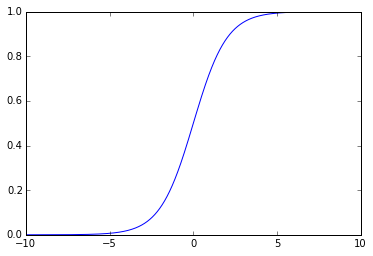
\includegraphics[scale=.5]{img/sigmoid_sat.png}
	\caption{Visualisation de la saturation de la fonction \emph{sigmoid} si
	$|z| \ge 5$.}
\end{figure} \\

Pour contrer cette saturation et donc accelerer les premi\`eres \'epoques
d'apprentissage, nous utiliserons une distribution plus \'etroite avec les
parametres $\mu=0$ et $\sigma =1/\sqrt{N}$ \\


\lstset{tabsize = 4,
frame=lines,
numbers=left,
captionpos=b,
caption = {Initialisation des poids et seuils},
language = python,
basicstyle=\small} \\
\begin{lstlisting}
self.biases  = [ np.random.randn(y, 1) for y in struct[1:] ]
self.weights = [ np.random.randn(y, x) / np.sqrt(x) \
				for x, y in zip(struct[:-1], struct[1:]) ]
\end{lstlisting}


\subsection{Fonctions d'activation}
% sigmoid  -> probability dist
% tanh     -> soft threshold (linear arround 0 hard threshold far)
% softplus -> linear above 0
% add plots



\subsection{Fonctions de cout}\label{cost}
% cross-entropy -> prevent neuron saturation
Comme ennonce precedemment, nous offrons aussi \`a l'utilisateur la possibilite
de choisir parmis differentes fonctions de couts, la fonctions que le reseau
cherche a minimiser en ajustant les poids et seuils des connections.
\paragraph{quadratic} est une
\href{https://fr.wikipedia.org/wiki/Erreur_quadratique_moyenne}
{fonction d'erreur quadratique moyenne}. Cete fonction est la plus simple et
est definie de la maniere suivante:
\begin{equation}
	\begin{aligned}
		C(w, b) &= \frac{1}{2\cdot d^{(L)}}\sum_{j}^{d^{(L)}}{({\bf\hat y} - {\bf y})^2}  \\
		{\bf C'}(w, b) &= \frac{1}{d^{(L)}}\cdot({\bf\hat y} - {\bf y})
	\end{aligned}
\end{equation}
\paragraph{cross-entropy} est la seconde option et est implementee dans le but
de limiter le phenomene de \emph{learning slowdown} en evitant la saturation des
neurones. Cette fonction permet au reseau de corriger ses poids plus efficacement
dans le cas d'une erreur importante. Elle ne peut etre seulement utilisee
avec une fonction d'activation \emph{sigmoid} et est construite pour annuler la
multiplication par $\sigma'(z)$ dans l'expression de $\boldsymbol\delta^{(L)}$.
\begin{equation}
	\begin{aligned}
		C(w, b) &= -\frac{1}{d^{(L)}}\sum_{j}^{d^{(L)}}{\left({\bf y}\ln({\bf\hat y}) +
		(1-{\bf y})\ln(1- {\bf \hat y})\right)}  \\
		{\bf C'}(w, b) &= \frac{1}{d^{(L)}}\cdot({\bf\hat y} - {\bf y})
	\end{aligned}
\end{equation}
NOTE: On remarque ici que les d\'eriv\'ees des deux fonctions sont identiques. En
revanche, une condition dans le code est ajout\'ee pour supprimer la multiplication
par $\sigma'(z)$.


\subsection{Eviter le sur-ajustement}\label{overfitting}
\begin{figure}[htp]
	\centering
	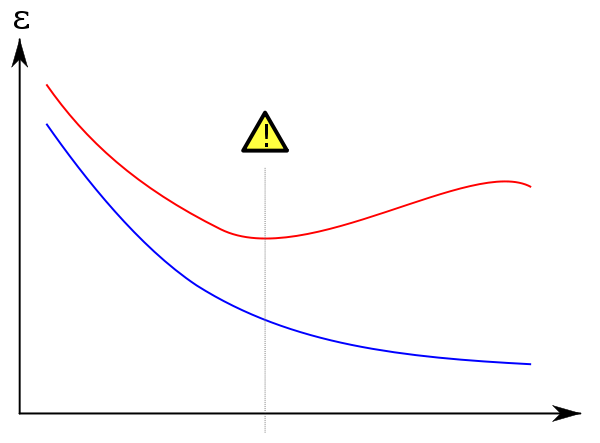
\includegraphics[scale=.4]{img/overfitting.png}
	\caption{erreurs sur le set d'entrainement(bleu) et de validation(rouge)}
\end{figure}
Le sur-ajustement (\emph{overfitting}) survient lorsque le reseau n'est plus
en train d'apprendre du dataset mais est en train de le m\'emoriser. Ceci se
traduit par un apprentissage trop sp\'ecifique aux donn\'ees, le reseau est
donc en train de modeliser le \emph{bruit}. Ceci survient lorsque le mod\`ele
(nombre de neurones et couches) est plus complexe que la fonction \`a
mod\'eliser. Ce sur-apprentissage a des consequences nefastes sur les
performances du reseau lorsqu'il est confronte a de nouvelles donnees il convient
donc de le detecter et de le minimiser.
\paragraph{Validation crois\'ee:} Pour detecter le sur-ajustement, il est
important de separer le set de donnees en deux une partie pour l'entrainement
l'autre pour la validation. Plusieurs methodes differentes sont disponibles
pour determiner comment separer le dataset. Plus on a de donnees dans le set
d'entrainement plus la prediction sera bonne mais moins on sera capable de
quantifier la capacit\'e de g\'en\'eralisation du r\'eseau et inversement.

Une methode interessante a citer est le \href{http://work.caltech.edu/slides/slides13.pdf}
{\emph{V-folds} ou \emph{K-folds}} qui permet de maximiser le nombre d'echantillons
d'entrainement en divisant le set complet en $V$ sous ensembles. Le reseau est
ensuite entrain\'e sur tous les sous-ensembles moins un qui est utilis\'e pour la
validation (le sous-ensemble de validation est choisi aleatoirement et change
a chaque epoque d'apprentissage). Il faut noter qu'il est important de
selectionner les echantillons de maniere aleatoire afin de ne pas biaiser
l'apprentissage du reseau.

Cependant, notre set de donnees etant deja separe en plusieurs sous-ensembles,
nous garderons ces methodes comme pistes d'amelioration futures.

\paragraph{Detection: }Le sur-ajustement peut etre aisement detecte lorsque
l'erreur sur le set de validation commence a augmenter tandis que l'erreur sur
le set d'entrainement continue de decroitre.
\paragraph{Early stopping} est une methode de limitation du sur-ajustement. Elle
consiste a monitorer les erreurs au cours de l'entrainement du reseau et
de l'interrompre sous certaines conditions(seuil, moyenne glissante, ...).

\paragraph{Les fonctions de r\'egularisation} sont une autre methode permettant
de limiter le sur-ajustement. Celles-ci ont pour approche de \emph{penaliser}
la minimisation de la fonction d'erreur dans le but d'ameliorer la capacite de
generalisation du reseau.

Ici, sont implement\'e deux des methodes les plus rependues :
r\'egularisation \emph{L1} et \emph{L2}. Toute deux visent a limiter
la magnitude poids dans l'ensemble du reseau.
Redefinissons la fonction de cout de la maniere suivante:
\begin{equation}
	\begin{aligned}
		C({\bf w}, {\bf b}) &= C_0({\bf w}, {\bf b}) + \Omega({\bf w})
	\end{aligned}
\end{equation}

O\`u $\Omega(w)$ est l'expression generale de la fonction de regularization.

On peut maintenant definir $\Omega({\bf w})$ pour chaque type de regularization:
\begin{equation}
	\begin{aligned}
		\Omega_{L1} ({\bf w}) &= \frac{\lambda}{2\cdot d^{(l)}} \cdot \sum{|{\bf w}^{(l)}|}\\
		\boldsymbol\Omega_{L1}'({\bf w}) &= \frac{\lambda}{d^{(l)}} \cdot sign\left ({\bf w}^{(l)} \right)\\
	\end{aligned}
\end{equation}
\begin{equation}
	\begin{aligned}
		\Omega_{L2} ({\bf w}) &= \frac{\lambda}{2\cdot d^{(l)}} \cdot \sum{\left({\bf w}^{(l)}\right) ^2}\\
		\boldsymbol\Omega_{L2}'({\bf w}) &= \frac{\lambda}{d^{(l)}} \cdot {\bf w}^{(l)}\\
	\end{aligned}
\end{equation}
NOTE: \href{http://work.caltech.edu/slides/slides12.pdf}{La r\'egularisation
\emph{Tikhonov}} est une forme generalis\'ee de ces approches et permet une
plus grande flexibilit\'e.


% penalise le poids large check :
% http://neuralnetworksanddeeplearning.com/chap3.html#overfitting_and_regularization

\subsection{Entrainement}
% batch gradient descent
% stochastic gradient descent
% minibatch GD check network.py

\subsection{Ajustement des hyper-param\`etres}
% http://neuralnetworksanddeeplearning.com/chap3.html#how_to_choose_a_neural_network's_hyper-parameters

\subsection{Inspection du res\'eau}

\section{Interface graphique}



\section{Discussions}
\subsection{Problemes rencontr\'es}
\subsection{Methodes de r\'esolution}
\subsection{conclusion et possibilites d'amelioration}
% ajouter autres pistes d'amelioration
% conclure sur performance globale du systeme
% classification homme/femme

\end{document}
% vim: cc=80 :
